\documentclass[10pt,twocolumn]{article}
\usepackage[margin=0.75in,columnsep=0.28in]{geometry}
\usepackage[T1]{fontenc}
\usepackage{amsmath,amssymb,amsthm}
\IfFileExists{lmodern.sty}{\usepackage{lmodern}}{}
\usepackage{booktabs,graphicx,array}
\IfFileExists{microtype.sty}{\usepackage[expansion=false]{microtype}}{}
\usepackage[colorlinks=true,linkcolor=blue,citecolor=blue,urlcolor=blue]{hyperref}
\setlength{\parskip}{2pt}
\sloppy

\newtheorem{proposition}{Proposition}
\newtheorem{lemma}{Lemma}
\theoremstyle{definition}
\newtheorem{definition}{Definition}
\newtheorem{remark}{Remark}

\newcommand{\Tten}{T_{10}}
\newcommand{\Pfive}{P_5}
\newcommand{\F}{\mathbb{F}_2}
\newcommand{\Hphys}{\mathcal{H}_{\mathrm{phys}}}
\newcommand{\Hedge}{\mathcal{H}_{\mathrm{edge}}}
\newcommand{\Hmicro}{H_{\mathrm{micro}}}
\newcommand{\PG}{P_G}
\newcommand{\XL}{X^{L}}
\newcommand{\tauc}{\tau_c^{(2)}}
% Release macros: written by generate_hashes.py into release_info.tex after the freeze.
\IfFileExists{release_info.tex}{\newcommand{\relName}{CCA-GaugeGraph-v1.9.2-frozen}
\newcommand{\relCommit}{5b38a1c35c74d042abba470a75cd8a7b\allowbreak 6a04b199}
\newcommand{\relSHA}{02a1b4e8f3b3706500ef55d014dc9130\allowbreak ff50b7c57498ef65f7eed4579b080eaa}
}{%
  \newcommand{\relName}{\textbf{[PRE-FREEZE BUILD]}}%
  \newcommand{\relCommit}{\textbf{[commit not yet minted]}}%
  \newcommand{\relSHA}{\textbf{[archive hash not yet minted]}}}

\title{\textbf{Gauge Constraints, Cycle Multiplicity, and\\ Finite-Graph Selection:\\ An Audited Computational and Perturbative Study}}
\author{Jake Riley\\ \small Independent Research Preprint\\ \small October 2026 \quad Version 1.9.2}
\date{}

\begin{document}
\twocolumn[
\maketitle
\begin{abstract}
\noindent This work studies a finite-graph mechanism in which cycle multiplicity, algebraic star-electric $\mathbb{Z}_2$ gauge constraints, and transverse quantum fluctuations contribute to geometry-dependent energetic weighting. The central methodological requirement is strict separation of four evidentiary classes: Class~A, exact analytic theorems within the stated finite model; Class~B, canonical numerical computations reproduced by a frozen computational pipeline; Class~C, finite-window empirical diagnostics; and Class~D, phenomenological attenuation assumptions. The microscopic Hamiltonian is $\Hmicro=-J\sum_e Z_e-g\sum_e X_e-K\sum_i Z_{\Gamma_i}$ with canonical parameters $J=1$, $K=0.5$, $g=0.15$. Around the fully polarized reference state a single-edge excitation has exact unperturbed gap $\Delta_e=2(J+Kk_e)$, where $k_e$ counts the selected basis cycles containing edge $e$. Exact star-electric Gauss projection gives $\PG Z_e\PG=0$, ${[X_e,\PG]}=0$ and $\PG X_e\PG=X_e\PG\neq0$, leaving a physical Hilbert space of dimension $2^{\beta_1}$. An independent cycle basis maps physical edge flips to binary logical translation masks; edges with equal columns (series classes, i.e.\ 2-edge cuts) give coherent amplitude multiplicities $m(\mathbf v)$ and hence $m(\mathbf v)^2$ second-order weights. For the canonical $\Tten$ versus $\Pfive$ comparison, a separately defined phenomenological attenuation model gives $\mathcal C_2(\Tten,\tau)=5.5+8e^{-2\tau}+9e^{-4\tau}$ and $\mathcal C_2(\Pfive)=10$, with exact crossing $u_c=(\sqrt{226}-8)/18$ for $u=e^{-2\tau}$ and $\tauc=0.4698581301779167\ldots$. The third-order XOR closure gives $\mathcal C_3(\Tten,\tau)=8+16e^{-\tau}+24e^{-3\tau}$ and a first-order displacement $a_1=-0.30954679241997696\ldots$, which a Richardson extrapolation of the finite-$g$ ladder reproduces to four digits. An arbitrary-precision (40-digit, confirmed at 60-digit) recomputation of the ladder shows that the binary64 roots carry noise of $4\times10^{-11}$ to $3\times10^{-8}$, and a linear Richardson extrapolation of the high-precision curvature gives $\hat a_{2,\mathrm{extrap}}\approx-8.404$, an empirical Class~C diagnostic. The unconstrained microscopic benchmark gives $E_0(T_8)<E_0(Q_3)<E_0(W_8)$. The conclusion is deliberately conditional: the finite model establishes an audited mechanism for cycle-incidence weighting and ordering of selected finite graph sectors under $H_A$, not a universal theory of geometric emergence.
\end{abstract}
\vspace{6pt}
]

%==========================================================
\section{Introduction}
The relation between graph topology, algebraic gauge constraints, and emergent effective structure is easy to overstate. A finite calculation can show that a specified Hamiltonian has a particular spectrum; it cannot, by itself, establish a universal physical principle. The present study is therefore built around a narrow and auditable question: can cycle multiplicity in a finite graph, after an exact $\mathbb Z_2$ star-electric projection, generate a calculable perturbative weighting whose attenuation can alter the energetic ordering of selected finite graph sectors under the effective Hamiltonian $H_A$?

The answer pursued here has four logically distinct layers. First, a microscopic Hamiltonian is specified on edge qubits. Second, its one-flip spectrum and exact Gauss projection are derived algebraically. Third, the physical Hilbert space is encoded by an independent cycle basis, so each physical edge flip becomes a binary logical translation. Fourth, an explicitly phenomenological attenuation law is imposed on repeated logical translations and its finite-size consequences are calculated. No step is silently promoted from one epistemic class to another.

The distinction matters because the unconstrained microscopic benchmark does not select the cubic graph $Q_3$. For the canonical parameters the frozen pipeline gives
\begin{align*}
E_0(T_8)&=-14.58250282755542,\\
E_0(Q_3)&=-14.575074400368777,\\
E_0(W_8)&=-14.568567641496603,
\end{align*}
so $T_8$ is lowest in energy. This is retained as a negative benchmark and is not adjusted to fit any intended geometric narrative.

The remainder of the paper develops the exact reduction, the multiplicity mechanism, the effective attenuation model, the analytic crossings, the finite-coupling numerical ladder, and the provenance architecture binding the published numbers to machine-readable fixtures.

%==========================================================
\section{Epistemic Structure and Scope}
Four epistemic classes are used. They classify the \emph{logical status} of a statement; how a number was obtained (analytic substitution or numerical root finding) is recorded separately in the manifest solver fields.
\begin{description}\setlength{\itemsep}{1pt}
\item[Class A: exact analytic results.] Closed derivations following from a stated finite mathematical model: the one-flip gap, Gauss-projection identities, the physical dimension, the logical encoding, and---conditionally on Class~D---the exact second-order crossing, the third-order XOR functional, and the first-order displacement. Results that depend on the attenuation ansatz are written Class~A$|$D.
\item[Class B: canonical numerical computations.] Finite-dimensional numerical results from the frozen pipeline with specified floating-point and solver conventions: the Rung-1 energies and the finite-$g$ crossing roots, in binary64 and in arbitrary-precision floating point.
\item[Class C: finite-window diagnostics.] Empirical quantities extracted from a finite numerical window or by extrapolation, namely the curvature estimates $\hat a_{2,\mathrm{extrap}}$ and $\hat a_{2,\mathrm{window}}$. These are not asymptotic theorems.
\item[Class D: phenomenological assumptions.] Modelling choices introduced after the exact layers, chiefly the attenuation factor $e^{-\tau(m-1)}$. They are not derived from the microscopic Hamiltonian.
\end{description}
The release-control hierarchy is
\[
\begin{aligned}\text{frozen source}&>\text{claim manifest}>\text{generated tables}\\&>\text{verification}>\text{draft prose}.\end{aligned}
\]
When two representations disagree, the higher-level artifact controls the release and the discrepancy is recorded. Numerical reproducibility is not mathematical interval certification, and neither is experimental validation.

The scope is finite: graphs are finite, connected and simple, and no thermodynamic or continuum limit is taken. The \emph{partition} of edges into multiplicity classes is basis independent (Proposition~\ref{prop:series}), but the mask labels, Hamming weights $|\mathbf v|$, and the cycle-parity terms depend on the chosen basis, so basis independence of the full effective model is not claimed. The attenuation law is a modelling ansatz.

%==========================================================
\section{Finite-Graph Framework}
Let $G=(V,E)$ be a finite connected simple graph with an edge qubit on every edge, $\Hedge=(\mathbb C^2)^{\otimes|E|}$. The cycle-space dimension over $\F$ is the first Betti number
\begin{equation}
\beta_1=|E|-|V|+1. \label{eq:beta}
\end{equation}
Choose an independent cycle basis $\mathcal B=\{\Gamma_1,\ldots,\Gamma_{\beta_1}\}$ with incidence matrix
\begin{equation}
B_{i,e}=\begin{cases}1,&e\in\Gamma_i,\\0,&e\notin\Gamma_i,\end{cases}\qquad B\in\F^{\beta_1\times|E|}, \label{eq:B}
\end{equation}
and cycle-parity operators
\begin{equation}
Z_{\Gamma_i}=\prod_{e\in\Gamma_i}Z_e. \label{eq:ZC}
\end{equation}
The basis is a computational object, part of the canonical fixture set, and is not claimed to be unique.

%==========================================================
\section{Microscopic Hamiltonian and One-Flip Gap}
The microscopic Hamiltonian is
\begin{equation}
\Hmicro=-J\sum_{e}Z_e-g\sum_{e}X_e-K\sum_{i=1}^{\beta_1}Z_{\Gamma_i}, \label{eq:Hmicro}
\end{equation}
with canonical values
\begin{equation}
J=1.0,\qquad K=0.5,\qquad g=0.15. \label{eq:params}
\end{equation}
At $g=0$ let $|0\rangle$ be the fully polarized $Z_e=+1$ state, with energy
\begin{equation}
E_0^{(0)}=-J|E|-K\beta_1. \label{eq:E0}
\end{equation}
Write $\Hmicro=H_0+V$ with $V=-g\sum_eX_e$ and $|e\rangle=X_e|0\rangle$. The flip raises the electric term on $e$ by $2J$, and every selected cycle containing $e$ changes its $Z_\Gamma$ eigenvalue from $+1$ to $-1$, raising the energy by $2K$ each. With
\begin{equation}
k_e=\sum_{i=1}^{\beta_1}B_{i,e}, \label{eq:ke}
\end{equation}
the exact unperturbed one-flip gap is
\begin{equation}
\Delta_e=2(J+Kk_e)\;\xrightarrow{\;J=1,\,K=0.5\;}\;2+k_e. \label{eq:gap}
\end{equation}
Because $\langle0|X_e|0\rangle=0$ the first-order correction vanishes, and the second-order Rayleigh--Schr\"odinger energy of the unconstrained model is
\begin{equation}
E_0^{(2)}=-g^2\sum_{e\in E}\frac{1}{2(J+Kk_e)}. \label{eq:E2micro}
\end{equation}
This belongs to the microscopic benchmark layer and must not be confused with the logical-mask functional of Sec.~\ref{sec:eff}. Finally, $U_Z=\prod_eZ_e$ satisfies $U_ZH(J,g,K)U_Z^\dagger=H(J,-g,K)$, so the microscopic ground-state energy is even in $g$ wherever the perturbation branch is analytic; in particular $E_0^{(3)}=0$ in the unconstrained model.

\textbf{Consistency check (Class A/B).} Using Eq.~\eqref{eq:E2micro} with $k_e$ from Table~\ref{tab:graphs}, $E_0^{(0)}+E_0^{(2)}$ equals $-14.58250$, $-14.57500$, $-14.56846$ for $T_8,Q_3,W_8$, against the numerical $-14.58250$, $-14.57507$, $-14.56857$ of Sec.~\ref{sec:rung1}; the residuals ($\lesssim10^{-4}$) are of the expected size $O(g^4)$.

%==========================================================
\section{Exact Star-Electric Gauss Projection}
For every vertex $v$ define
\begin{equation}
G_v=\prod_{e\in\mathrm{star}(v)}X_e. \label{eq:Gv}
\end{equation}
All $G_v$ commute, being products of Pauli-$X$ operators. Since every edge has exactly two endpoints,
\begin{equation}
\prod_{v\in V}G_v=\mathbb I. \label{eq:prodG}
\end{equation}
For a connected graph this is the \emph{only} relation among the $G_v$: the $G_v$ correspond to the vertex stars $\delta_v\in\F^{E}$, which span the cut space, of dimension $|V|-1$. These $G_v$ are stabilizer-type constraints on edge qubits; no continuum gauge-field interpretation and no physical spacetime gauge theory is assumed anywhere in this work. Fix a reference vertex $v_0$ and define
\begin{equation}
\begin{gathered}\PG=\prod_{v\neq v_0}\frac{\mathbb I+G_v}{2},\\ \Hphys=\PG\Hedge=\{|\psi\rangle:G_v|\psi\rangle=|\psi\rangle\ \forall v\}.\end{gathered} \label{eq:PG}
\end{equation}
By Eq.~\eqref{eq:prodG}, $G_{v_0}=\prod_{v\ne v_0}G_v$, hence $\PG G_{v_0}=\PG$ as well; therefore $\PG G_u=G_u\PG=\PG$ for \emph{every} $u\in V$, including $u=v_0$. This closes the one step that Eq.~\eqref{eq:PG} alone does not display.

\subsection{Longitudinal edge operator}
For $e=(u,v)$, $Z_e$ anticommutes with $G_u$ and $G_v$. Using $G_uZ_e=-Z_eG_u$ and $\PG G_u=G_u\PG=\PG$,
\[
\PG Z_e\PG=\PG G_uZ_eG_u\PG=-\PG Z_e\PG,
\]
hence
\begin{equation}
\PG Z_e\PG=0. \label{eq:PZP}
\end{equation}

\subsection{Transverse edge operator}
Each $G_v$ is a product of $X$ operators, so $[X_e,G_v]=0$ for all $v,e$ and
\begin{equation}
[X_e,\PG]=0,\qquad \PG X_e\PG=X_e\PG=\PG X_e\neq0. \label{eq:PXP}
\end{equation}
Non-vanishing follows because $X_e$ is unitary and maps $\Hphys$ to itself; $X_e\PG$ acts as a unitary on $\Hphys\neq\{0\}$. The projection removes the bare longitudinal link term and preserves the gauge-invariant transverse transition.

\subsection{Physical dimension}
Since $|V|-1$ independent commuting $\pm1$ constraints each halve the space,
\begin{equation}
\dim\Hphys=2^{|E|-(|V|-1)}=2^{\beta_1}, \label{eq:dim}
\end{equation}
in agreement with the rank of the binary cycle space, Eq.~\eqref{eq:beta}.

%==========================================================
\section{Logical Cycle-Flux Encoding and Multiplicity}
\subsection{The logical isometry}
Work in the $Z$-basis $|s\rangle$, $s\in\F^{E}$ ($s_e=1$ meaning $Z_e=-1$). Then $G_v|s\rangle=|s+\delta_v\rangle$, so gauge orbits are cosets $s+\mathcal C^\perp$ of the cut space $\mathcal C^\perp=\mathrm{span}\{\delta_v\}$, and a physical basis state is the uniform superposition
\[
|[s]\rangle=2^{-(|V|-1)/2}\sum_{c\in\mathcal C^\perp}|s+c\rangle .
\]
Over $\F$ the cycle space and cut space are mutually orthogonal complements, and the rows of $B$ span the cycle space, so $\ker B=\mathcal C^\perp$. Hence $s\mapsto Bs\in\F^{\beta_1}$ labels the cosets bijectively, and $|[s]\rangle\mapsto|Bs\rangle$ defines a unitary $U:\Hphys\to(\mathbb C^2)^{\otimes\beta_1}$. The label bits are exactly the cycle parities: $Z_{\Gamma_i}|[s]\rangle=(-1)^{(Bs)_i}|[s]\rangle$, i.e.\ $U Z_{\Gamma_i}U^\dagger=\bar Z_i$.

Now $X_e|[s]\rangle=|[s+\mathbf e_e]\rangle$ and $B(s+\mathbf e_e)=Bs+\mathbf b_e$ with
\begin{equation}
\mathbf b_e=B_{*,e}\in\F^{\beta_1}. \label{eq:be}
\end{equation}
Therefore, with $\XL(\mathbf v)=\prod_{i:v_i=1}\bar X_i$,
\begin{equation}
U(\PG X_e\PG)U^\dagger=\XL(\mathbf b_e). \label{eq:iso}
\end{equation}
This is a proof (Class A), not an assumption.

\subsection{Multiplicity as series classes}
\begin{definition}
For nonzero $\mathbf v\in\F^{\beta_1}$, $m(\mathbf v)=\#\{e\in E:\mathbf b_e=\mathbf v\}$.
\end{definition}
\begin{proposition}\label{prop:series}
For $e\neq e'$, $\mathbf b_e=\mathbf b_{e'}$ if and only if $\mathbf e_e+\mathbf e_{e'}\in\ker B=\mathcal C^\perp$, i.e.\ iff $\{e,e'\}$ is a cut of $G$ (a 2-edge cut if neither edge is a bridge, i.e.\ $e,e'$ lie in exactly the same cycles). In that case $X_e=X_{e'}$ on $\Hphys$.
\end{proposition}
\begin{proof}
$\mathbf b_e+\mathbf b_{e'}=B(\mathbf e_e+\mathbf e_{e'})$, which vanishes iff $\mathbf e_e+\mathbf e_{e'}\in\ker B=\mathcal C^\perp$. Then $\mathbf e_e+\mathbf e_{e'}=\sum_{v\in S}\delta_v$ for some vertex set $S$, so $X_eX_{e'}=\prod_{v\in S}G_v$, which acts as the identity on $\Hphys$.
\end{proof}
The simplest instance is two edges meeting at a degree-2 vertex; longer subdivided paths and genuine 2-edge cuts also qualify. The \emph{partition} of non-bridge edges into series classes is intrinsic to $G$ and independent of the cycle basis, because $\ker B=\mathcal C^\perp$ for every basis. What does depend on the basis is the labelling $\mathbf v$, its Hamming weight $|\mathbf v|$, and the cycle-parity term in Eq.~\eqref{eq:Hmicro}. A bridge has $\mathbf b_e=\mathbf 0$ and $X_e=\mathbb I$ on $\Hphys$; it is excluded from all sums below, which run over the occupied set $\mathcal V=\{\mathbf v\neq0:m(\mathbf v)>0\}$.

\textbf{Coherent addition.} If $m(\mathbf v)$ distinct edges yield the same logical operator, their amplitudes add: $-g\,\XL(\mathbf v)$ becomes $-g\,m(\mathbf v)\XL(\mathbf v)$ before attenuation, and the second-order weight is
\begin{equation}
\bigl(g\,m(\mathbf v)\bigr)^2=g^2m(\mathbf v)^2. \label{eq:m2}
\end{equation}
The factor $m^2$ is thus an amplitude-addition consequence of the logical representation, not a phenomenological assertion. Since distinct edges in a series class act identically on $\Hphys$, the $m^2$ weighting is the statement that a subdivided link behaves as one coherent link.

%==========================================================
\section{Canonical Graph Set}
The frozen baseline contains five graphs. Edge counts and Betti numbers follow from Eq.~\eqref{eq:beta}; the $k_e$ distributions come from the canonical bases of Appendix~B.

\begin{table}[h]
\centering\small
\caption{Canonical graph sizes, cycle ranks, and $k_e$ multiplicities ($a^{n}$ means $n$ edges with $k_e=a$).}
\label{tab:graphs}
\begin{tabular}{@{}lcccrl@{}}
\toprule
Graph&$|V|$&$|E|$&$\beta_1$&$\sum_ek_e$&distribution\\\midrule
$T_8$&8&12&5&16&$1^8,2^4$\\
$Q_3$&8&12&5&20&$1^4,2^8$\\
$W_8$&8&12&5&28&$1^5,2^2,3^2,4^2,5^1$\\
$T_{10}$&10&15&6&20&$1^{10},2^5$\\
$P_5$&10&15&6&25&$1^5,2^{10}$\\\bottomrule
\end{tabular}
\end{table}
The sum $\sum_ek_e$ equals the total number of edge occurrences across the basis cycles, a basis-level consistency check (e.g.\ for $W_8$: $5+5+5+5+8=28$).

%==========================================================
\section{Rung-1 Microscopic Numerical Benchmark}\label{sec:rung1}
Equation~\eqref{eq:Hmicro} is diagonalized on the full edge-qubit space for $T_8,Q_3,W_8$ at $J=1$, $K=0.5$, $g=0.15$, using sparse symmetric Lanczos (ARPACK) with a deterministic uniform start vector, a residual check, and binary64 arithmetic.

\begin{table}[h]
\centering\small
\caption{Canonical Rung-1 ground-state energies (Class B).}
\begin{tabular}{@{}lr@{}}
\toprule Graph&$E_0$\\\midrule
$T_8$&$-14.58250282755542$\\
$Q_3$&$-14.575074400368777$\\
$W_8$&$-14.568567641496603$\\\bottomrule
\end{tabular}
\end{table}
The frozen residual norms are $3.39\times10^{-14}$, $1.13\times10^{-13}$ and $3.18\times10^{-14}$. The ordering is
\begin{equation}
E_0(T_8)<E_0(Q_3)<E_0(W_8), \label{eq:order}
\end{equation}
which withdraws any earlier claim that the unconstrained benchmark favours $Q_3$.

\textbf{Basis sensitivity of the benchmark.} Because the $K$-term of Eq.~\eqref{eq:Hmicro} sums over a chosen cycle basis, $\Hmicro$ itself depends on that choice. The canonical bases of $T_8$, $Q_3$, $\Tten$ and $\Pfive$ are minimum-total-length cycle bases (total edge-length $16$, $20$, $20$, $25$, equal to the minimum over all bases), but the canonical $W_8$ basis is not ($28$ against a minimum of $21$). Replacing it by a minimum-length basis (cycles $\{0,4,8,9\}$, $\{1,5,9,10\}$, $\{3,7,8,11\}$, $\{2,6,10,11\}$, $\{0,1,2,3,8\}$ in the edge indexing of Appendix~A) gives $E_0(W_8)=-14.573955882390418$ (residual $1.2\times10^{-14}$; CLM-015). The ordering of Eq.~\eqref{eq:order} is unchanged, but the $W_8$ energy shifts by $-5.39\times10^{-3}$, so the benchmark values are conditional on the stated bases. The minimum-length basis is not unique; the one used is the deterministic greedy choice, and its cycles are verified to be simple and to span the same cycle space as the canonical basis.

\textbf{Ground-state certification.} A small residual shows only that the returned value is close to \emph{an} eigenvalue. In the $Z$-basis all off-diagonal elements of Eq.~\eqref{eq:Hmicro} equal $-g<0$ and the edge-flip graph is connected, so by Perron--Frobenius the ground state is nondegenerate with strictly positive components. A positive start vector (the uniform vector used here) therefore has nonzero overlap with it, which is the property that makes Lanczos converge to the lowest eigenvalue. This is an argument for the correctness of the target, not an independent numerical certificate.

\begin{figure}[t]
\centering
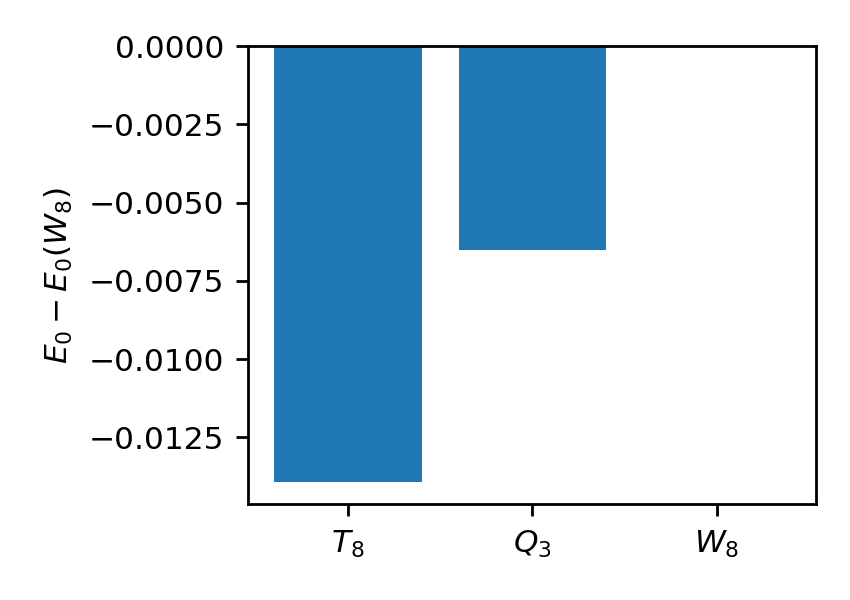
\includegraphics[width=0.8\columnwidth]{fig1.png}
\caption{Rung-1 energies relative to $W_8$, $\Delta E_0=E_0-E_0(W_8)$. The ordering $T_8<Q_3<W_8$ is explicit.}
\end{figure}

\subsection*{Microscopic benchmark on $\Tten$ and $\Pfive$}
To place the microscopic and effective calculations on the same graphs, the archived pipeline applies the same sparse Lanczos procedure (same $J,K,g$, bases of Appendix~B, uniform start vector) to all five graphs. For $T_8$, $Q_3$ and $W_8$ it reproduces the canonical energies above to within $3\times10^{-14}$. For $\Tten$ and $\Pfive$ ($2^{15}=32768$ states) it gives
\begin{align}E_0(\Tten)&=-18.103159053426,\\ E_0(\Pfive)&=-18.093856286849, \label{eq:micro1015}\end{align}
so $E_0(\Tten)<E_0(\Pfive)$ (Class~B, CLM-016). These values bridge the microscopic and effective calculations by placing both on the same pair of graphs; they leave the attenuation ansatz itself untouched. The microscopic ordering does not test the attenuation mechanism, because $H_A$ of the next section is an independent effective model (Sec.~\ref{sec:eff}).

%==========================================================
\section{Phenomenological Attenuated Effective Model}\label{sec:eff}
\textbf{The break with the microscopic model.} By Eq.~\eqref{eq:PZP} the term $J\sum_eZ_e$ vanishes identically under projection onto $\Hphys$; it is gauge-variant, does not preserve $\Hphys$, and the gaps of Eq.~\eqref{eq:gap} do not survive restriction. Consequently $P_G\Hmicro P_G$ is not a faithful reduction of $\Hmicro$ to the logical space, and the effective Hamiltonian below \emph{cannot} be derived by unitary projection. It is introduced as an independent logical model. Likewise, $U_Z$ maps $G_v\mapsto(-1)^{\deg v}G_v$, so it does not preserve $\Hphys$ when $G$ has odd-degree vertices, and $H_A$ has no $g\to-g$ symmetry; odd orders such as $E^{(3)}$ therefore need not vanish in the effective model, and the third-order term that drives $a_1$ is present only there.

The effective Hamiltonian is
\begin{equation}
H_A(\tau)=-K\sum_{i=1}^{\beta_1}\bar Z_i-g\sum_{\mathbf v\in\mathcal V}a(\mathbf v,\tau)\,\XL(\mathbf v), \label{eq:HA}
\end{equation}
with the attenuation factor
\begin{equation}
a(\mathbf v,\tau)=m(\mathbf v)\,e^{-\tau[m(\mathbf v)-1]}. \label{eq:a}
\end{equation}
This is a \textbf{Class~D} ansatz: it is not derived from Eq.~\eqref{eq:Hmicro}, from the Gauss projection, or from the graph-theoretic identities above. It poses a controlled question: what happens if repeated logical transitions are increasingly attenuated as multiplicity rises?

Flipping logical coordinates $\mathbf v$ from the reference sector changes $|\mathbf v|$ cycle parities, so the excitation gap is $\Delta_{\mathbf v}=2K|\mathbf v|$, equal to $|\mathbf v|$ at $K=\tfrac12$. The perturbation expansion of $H_A$ about the logical reference state gives $E^{(1)}=0$ and
\begin{align}
E^{(2)}&=-g^2\,\mathcal C_2(G,\tau), \qquad E^{(3)}=-g^3\,\mathcal C_3(G,\tau),\label{eq:E23}\\
\mathcal C_2(G,\tau)&=\sum_{\mathbf v\in\mathcal V}\frac{a(\mathbf v,\tau)^2}{|\mathbf v|}, \label{eq:C2}\\
\mathcal C_3(G,\tau)&=\sum_{\substack{\mathbf u,\mathbf w,\mathbf r\in\mathcal V\\ \mathbf u\oplus\mathbf w\oplus\mathbf r=0}}\frac{a(\mathbf u)a(\mathbf w)a(\mathbf r)}{|\mathbf u|\,|\mathbf r|}. \label{eq:C3}
\end{align}
In Eq.~\eqref{eq:C3} the sum runs over \emph{ordered} paths $0\to\mathbf u\to\mathbf u\oplus\mathbf w=\mathbf r\to0$; the two intermediate states carry excitation energies $|\mathbf u|$ and $|\mathbf r|$, so these---not $|\mathbf w|$---appear in the denominator. The term $-E^{(1)}\sum|\langle a|V|0\rangle|^2/\Delta^2$ in third-order theory vanishes since $E^{(1)}=0$. The overall sign follows from $(-g)^3/[(+\Delta_{\mathbf u})(+\Delta_{\mathbf r})]$ with energy denominators $E^{(0)}-E_a=-\Delta_a$.

\textbf{General $K$.} For arbitrary $K$, $\mathcal C_2\to\mathcal C_2/(2K)$ and $\mathcal C_3\to\mathcal C_3/(2K)^2$. The second-order threshold $\tauc$ is $K$-independent, while $a_1\to a_1/(2K)$. All numerical values below are at $K=\tfrac12$. The two functionals compared have equal $\beta_1$ (both $6$), so the reference energy $-K\beta_1$ cancels in differences.

Equations~\eqref{eq:C2}--\eqref{eq:C3} are reduced functionals after the exact gauge encoding and the Class~D assumption; they must not be identified with Eq.~\eqref{eq:E2micro}.

%==========================================================
\section{Canonical $\Tten$ Mask Spectrum}
The graph $\Tten$ has six independent cycles and fifteen edges. The columns of its $6\times15$ incidence matrix (Appendix~C) give eleven distinct nonzero masks, written as integers in the binary-coordinate convention of the fixture:
\begin{equation}
\{1,2,3,4,6,8,12,16,24,32,48\}. \label{eq:masks}
\end{equation}
Their multiplicities are
\begin{equation}
\{2,1,1,1,1,1,1,2,1,3,1\}, \label{eq:mult}
\end{equation}
so the multiplicity multiset is $\{1^8,2^2,3^1\}$, summing to $8+4+3=15$ edges.
\begin{table}[h]
\centering\footnotesize
\caption{Canonical $\Tten$ logical masks.}
\setlength{\tabcolsep}{3pt}
\begin{tabular}{@{}lccccccccccc@{}}
\toprule
$\mathbf v$&1&2&3&4&6&8&12&16&24&32&48\\\midrule
$m$&2&1&1&1&1&1&1&2&1&3&1\\
$|\mathbf v|$&1&1&2&1&2&1&2&1&2&1&2\\\bottomrule
\end{tabular}
\end{table}
The eight singly represented masks contribute $\sum 1/|\mathbf v|=5.5$; the two multiplicity-two masks contribute $4(1/1+1/1)e^{-2\tau}=8e^{-2\tau}$; the multiplicity-three mask contributes $9e^{-4\tau}$. Thus
\begin{equation}
\mathcal C_2(\Tten,\tau)=5.5+8e^{-2\tau}+9e^{-4\tau}. \label{eq:C2T}
\end{equation}
For $\Pfive$ all fifteen nonzero columns are distinct ($m\equiv1$), giving
\begin{equation}
\mathcal C_2(\Pfive)=10, \label{eq:C2P}
\end{equation}
and at zero attenuation $\mathcal C_2(\Tten,0)=22.5$.

%==========================================================
\section{Exact Second-Order Crossing}
Set $u=e^{-2\tau}$. Equating Eqs.~\eqref{eq:C2T} and \eqref{eq:C2P},
\begin{equation}
18u^2+16u-9=0 .\label{eq:quad}
\end{equation}
The roots are $(-8\pm\sqrt{226})/18$; only the positive root is admissible since $u>0$:
\begin{align}
u_c&=\frac{\sqrt{226}-8}{18}=0.3907386876873838\ldots,\label{eq:uc}\\
\tauc&=-\tfrac12\ln u_c=0.4698581301779167\ldots.\label{eq:tauc}
\end{align}
This is Class~A$|$D: exact within the explicitly defined effective model.

\begin{figure}[t]
\centering
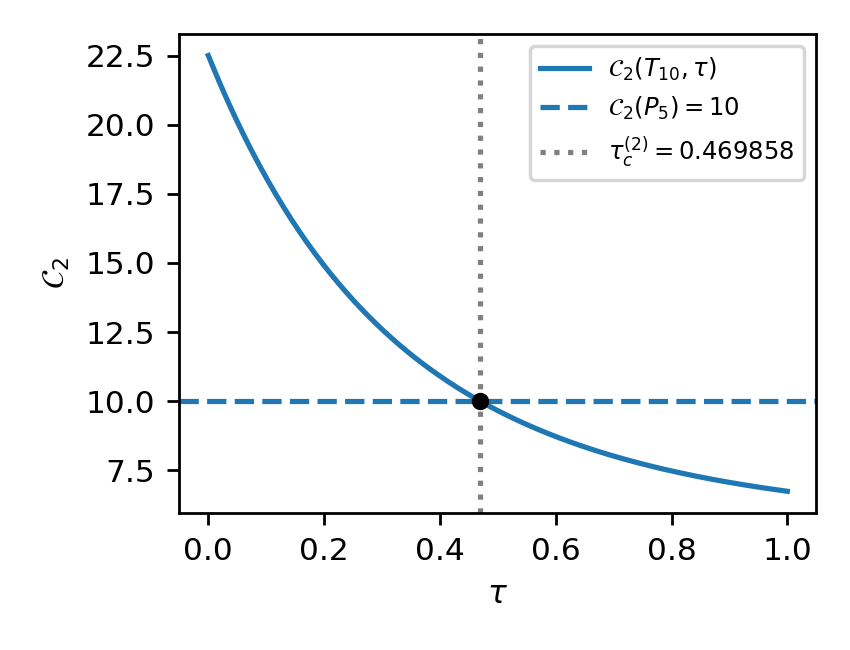
\includegraphics[width=0.8\columnwidth]{fig2.png}
\caption{Second-order effective crossing: $\mathcal C_2(\Tten,\tau)$ meets the constant $\mathcal C_2(\Pfive)=10$ at $\tauc$.}
\end{figure}

\subsection{Dependence on the cycle basis}\label{sec:basisdep}
The multiplicities $m(\mathbf v)$ are basis independent as a partition (Proposition~\ref{prop:series}), but the Hamming weights $|\mathbf v|$ in Eq.~\eqref{eq:C2} are not invariant under a change of basis $B\mapsto MB$, $M\in GL(\beta_1,\F)$. Permutations of the basis coordinates leave $\mathcal C_2$ unchanged; general $M$ do not. To quantify this, $20{,}000$ pairs of independent bases were drawn uniformly from $GL(6,\F)$ (one for $\Tten$, one for $\Pfive$, by rejection sampling of invertible matrices; fixed seed), the masks transformed by $\mathbf v\mapsto M\mathbf v$ with multiplicities unchanged, and $\mathcal C_2$ and the crossing recomputed. The results (an empirical sampling test, Class~C, CLM-014) are:
\begin{itemize}\setlength{\itemsep}{0pt}
\item $\mathcal C_2(\Tten,0)$ ranges over $5.8$--$20.9$ (median $9.5$) and $\mathcal C_2(\Pfive)$ over $4.1$--$9.5$ (median $6.0$). The canonical values $22.5$ and $10$ lie above every sample, because the canonical bases consist of short cycles and give sparse, low-weight masks.
\item A second-order crossing exists in $98.8\%$ of the draws. Where it exists, $\tau_c$ has 5th, 50th and 95th percentiles $0.08$, $0.30$ and $0.64$, against the canonical $0.4699$.
\end{itemize}
The qualitative crossing is therefore robust, but the numerical threshold $\tauc$ is not an invariant of the graph: it is conditional on a principled basis rule. A natural rule is a minimum-total-length cycle basis. For $\Tten$ and $\Pfive$ the canonical bases already satisfy it, and $3000$ draws of minimum-length bases with random tie-breaking (random-order greedy) all gave $\mathcal C_2(\Tten,0)=22.5$, $\mathcal C_2(\Pfive)=10$ and $\tau_c^{(2)}=0.4699$. This is empirical support that the functional is constant on the sampled minimum-length bases; invariance over all of them is not proved. The results of Secs.~\ref{sec:eff}--\ref{sec:ladder} are stated for these bases.

%==========================================================
\section{Third-Order XOR Closure}
The third-order functional depends on triples of occupied masks with $\mathbf v_1\oplus\mathbf v_2\oplus\mathbf v_3=0$. Among the $\binom{11}{3}=165$ triples of distinct $\Tten$ masks, exact enumeration gives five closures:
\begin{equation}
\{1,2,3\},\ \{2,4,6\},\ \{4,8,12\},\ \{8,16,24\},\ \{16,32,48\}.\label{eq:xor}
\end{equation}
Each has Hamming weights $(1,1,2)$. For a closure with weights $(1,1,2)$ the six ordered assignments $(\mathbf u,\mathbf w,\mathbf r)$ contribute $\sum1/(|\mathbf u||\mathbf r|)=2\cdot1+4\cdot\tfrac12=4$ times $a(\mathbf v_1)a(\mathbf v_2)a(\mathbf v_3)$. The attenuation products are $2e^{-\tau}$, $1$, $1$, $2e^{-\tau}$, $6e^{-3\tau}$, hence
\begin{equation}
\mathcal C_3(\Tten,\tau)=8+16e^{-\tau}+24e^{-3\tau}. \label{eq:C3T}
\end{equation}
For $\Pfive$ there are ten closures: five with weights $(1,1,2)$, contributing $5\times4=20$, and five with weights $(2,2,2)$, each contributing $6\cdot\tfrac14=\tfrac32$, i.e.\ $7.5$. Thus
\begin{equation}
\mathcal C_3(\Pfive)=27.5. \label{eq:C3P}
\end{equation}
At the second-order threshold
\begin{align}
\mathcal C_3(\Tten,\tauc)&=23.86338825560875\ldots,\\
\Delta\mathcal C_3&=-3.636611744391253\ldots,\label{eq:dC3}
\end{align}
where $\Delta\mathcal C_3=\mathcal C_3(\Tten,\tauc)-\mathcal C_3(\Pfive)$.
The bookkeeping quantities must remain distinct: $\mathcal C_2(\Tten,0)=22.5$; $\mathcal C_3(\Tten,0)=8+16+24=48$; $\mathcal C_3(\Tten,\tauc)=23.863\ldots$. The historical value $23$ in an earlier draft was a bookkeeping error and is not used.

%==========================================================
\section{Analytic First-Order Crossing Displacement}
The energy difference of the two effective sectors is
\[
\begin{aligned}\Delta E(\tau,g)=&-g^2\bigl[\mathcal C_2(\Tten,\tau)-\mathcal C_2(\Pfive)\bigr]\\&-g^3\bigl[\mathcal C_3(\Tten,\tau)-\mathcal C_3(\Pfive)\bigr]+O(g^4).\end{aligned}
\]
Dividing $\Delta E=0$ by $g^2$ and writing $\tau_c(g)=\tauc+a_1g+a_2g^2+\cdots$,
\begin{equation}
\mathcal C_2'(\tauc)\,a_1+\Delta\mathcal C_3=0 ,\label{eq:cross1}
\end{equation}
with $\mathcal C_2'(\tau)=-16e^{-2\tau}-36e^{-4\tau}$ and $\mathcal C_2'(\tauc)=-11.74818099700186\ldots$. Hence
\begin{equation}
a_1=-\frac{\Delta\mathcal C_3}{\mathcal C_2'(\tauc)}=-0.30954679241997696\ldots.\label{eq:a1}
\end{equation}
This is Class~A$|$D within the effective model; it is not fitted to the numerical ladder. It rests on truncation at third order and presumes analyticity of the perturbation branch near $\tauc$. The next coefficient $a_2$ is not derived analytically; it is estimated numerically in Sec.~\ref{sec:ladder}.

%==========================================================
\section{Canonical Finite-$g$ Crossing Ladder}\label{sec:ladder}
The finite-$g$ comparison is evaluated in the six-logical-qubit space. For $\Tten$ the eleven masks and multiplicities are used; for $\Pfive$ the fifteen masks with unit multiplicity. The matrices are real symmetric $64\times64$; lowest eigenvalues are computed in IEEE-754 binary64 and the crossing is located by a bracketed Brent solver with $\mathrm{xtol}=10^{-14}$, $\mathrm{rtol}=4\epsilon_{\mathrm{mach}}$, $\epsilon_{\mathrm{mach}}=2.220446049250313\times10^{-16}$. The binary64 roots are reproducible outputs of a specified computation, not rigorous interval enclosures. The ladder is additionally recomputed in arbitrary-precision floating point (mpmath 1.3.0, 40 digits, eigenvalues by \texttt{eigsy}, secant-type root search with tolerance $10^{-30}$), and the five roots are confirmed by a 60-digit run (tolerance $10^{-45}$) to at least 24 digits. These are floating-point results, not interval enclosures. Define $\hat a_2(g)=\bigl([\tau_c-\tauc]/g-a_1\bigr)/g$.

\begin{table*}[t]
\centering\small
\caption{Finite-$g$ crossing ladder. The high-precision root (40 digits, confirmed at 60) is the Class~B reference, quoted to 12 decimals. The binary64 column is the canonical pipeline output; ``difference'' is binary64 minus high precision. Historical values are retained for provenance only. $\hat a_2(g)=([\tau_c-\tauc]/g-a_1)/g$ is evaluated from the high-precision roots.}
\label{tab:ladder}
\begin{tabular}{@{}lllrrr@{}}
\toprule
$g$&high-precision $\tau_c$&binary64 canonical&difference&historical&$\hat a_2(g)$\\\midrule
0.0020&0.469205151252&0.4692051514033929&$+1.5\times10^{-10}$&0.4692051513802&$-8.47134$\\
0.0010&0.469540145720&0.4695401454094673&$-3.1\times10^{-10}$&0.4695401454379&$-8.43767$\\
0.0005&0.469701251573&0.4697012515365259&$-3.6\times10^{-11}$&0.4697012508551&$-8.42083$\\
0.0002&0.469795884390&0.4697958818370814&$-2.6\times10^{-9}$&0.4697958758557&$-8.41074$\\
0.0001&0.469827091425&0.4698270588560223&$-3.3\times10^{-8}$&0.4698270714617&$-8.40737$\\\bottomrule
\end{tabular}
\end{table*}

The high-precision $\hat a_2(g)$ varies smoothly and monotonically across the whole ladder. If $\hat a_2(g)=a_2+a_3g+\cdots$, linear Richardson extrapolation $2\hat a_2(g)-\hat a_2(2g)$ applied to two independent pairs gives
\begin{align}
(g=0.0001,\,0.0002):&\ -8.40401,\nonumber\\
(g=0.0005,\,0.001):&\ -8.40400,\nonumber
\end{align}
which agree to five digits, so
\begin{equation}
\hat a_{2,\mathrm{extrap}}\approx-8.404 .\label{eq:a2extrap}
\end{equation}
This is \textbf{Class~C}: an empirical extrapolation that assumes an analytic expansion with a linear leading correction, not an asymptotic theorem. The mean of $\hat a_2$ over the window $g\in[0.0005,0.002]$ is a secondary descriptive statistic: it is $-8.44328$ from the high-precision roots (the binary64 pipeline reports $-8.443418057955176$). It is biased by about $0.04$ relative to Eq.~\eqref{eq:a2extrap} because the window lies at larger $g$.

\textbf{Validation of $a_1$.} Linear Richardson extrapolation of $[\tau_c-\tauc]/g$ to $g\to0$ from the high-precision $g=0.0005$ and $0.001$ rows gives $-0.30953$, against the analytic $a_1=-0.309547$. This agreement (to $\sim2\times10^{-5}$) is the principal quantitative cross-check between the Class~A$|$D prediction and Class~B computation.

\begin{figure}[t]
\centering
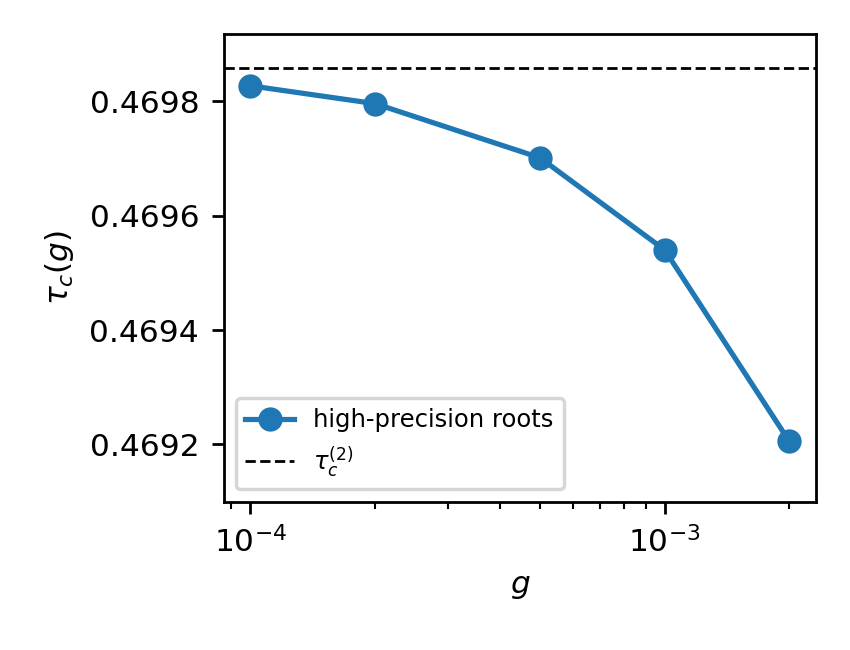
\includegraphics[width=0.8\columnwidth]{fig3.png}
\caption{Finite-$g$ crossing ladder approaching $\tauc$ as $g\to0$. High-precision Class~B roots; the dashed line is $\tauc$.}
\end{figure}

\subsection{Historical root-finding discrepancy and numerical noise}
To test whether the erratic behaviour at $g\le2\times10^{-4}$ reflects binary64 cancellation, the crossing was recomputed with 40-digit arithmetic and confirmed at 60 digits. The canonical binary64 roots differ from the high-precision roots by $4\times10^{-11}$ to $3\times10^{-8}$, bounded by an envelope growing roughly as $g^{-2}$ as expected from the eigenvalue-noise estimate. The high-precision $\hat a_2(g)$ varies smoothly. This is arbitrary-precision floating-point evidence, not an interval enclosure.

The expected envelope follows from $\Delta E\approx g^2|\mathcal C_2'|\,\delta\tau$: an absolute eigenvalue error $\delta E\sim10^{-15}$ limits the binary64 root to
\begin{equation}
\delta\tau\sim\frac{\delta E}{g^2|\mathcal C_2'(\tauc)|},
\end{equation}
about $3\times10^{-10}$ at $g=5\times10^{-4}$ and $10^{-8}$ at $g=10^{-4}$. The noise is random, not monotone in $g$ (the $g=0.0005$ root is closer to the reference than the $g=0.001$ root), so this is an envelope and not a fit. The archived pipeline builds $H_A$ from the definitions in Sec.~\ref{sec:eff}; its binary64 roots are recomputed in the verification suite and agree with the original v1.9 canonical roots within this envelope.

For the historical $g=0.0005$ value $0.4697012508551$, the high-precision reference is $0.4697012515730$, so the historical root is off by $7.2\times10^{-10}$ and the tightened canonical root by only $3.6\times10^{-11}$. The tightened calculation is therefore the more accurate of the two, but this comparison does not identify whether the historical error came from solver tolerance or from eigenvalue noise. Neither affects $\tauc$ or $a_1$.

%==========================================================
\section{Manifest Claim Ledger}
The release manifest contains sixteen named claims. Class labels follow Sec.~2.
\begin{description}\setlength{\itemsep}{0pt}\small
\item[CLM-001] $E_0(T_8)$; Class B; canonical; $-14.58250282755542$; residual $3.39\times10^{-14}$.
\item[CLM-002] $E_0(Q_3)$; Class B; canonical; $-14.575074400368777$; residual $1.13\times10^{-13}$.
\item[CLM-003] $E_0(W_8)$; Class B; canonical; $-14.568567641496603$; residual $3.18\times10^{-14}$.
\item[CLM-004] $u_c$; Class A$|$D; canonical; $(\sqrt{226}-8)/18=0.3907386876873838\ldots$.
\item[CLM-005] $\tauc$; Class A$|$D; canonical; $-\tfrac12\ln[(\sqrt{226}-8)/18]=0.4698581301779167\ldots$.
\item[CLM-006] $a_1$; Class A$|$D; canonical; $-\Delta\mathcal C_3/\mathcal C_2'=-0.30954679241997696\ldots$, with $\mathcal C_2'=-11.74818099700186\ldots$, $\Delta\mathcal C_3=-3.636611744391253\ldots$.
\item[CLM-007] $\tau_c(g{=}0.0020)$; Class B; high-precision reference $0.469205151252$; binary64 canonical $0.4692051514033929$; historical $0.4692051513802$.
\item[CLM-008] $\tau_c(g{=}0.0010)$; Class B; high-precision reference $0.469540145720$; binary64 canonical $0.4695401454094673$; historical $0.4695401454379$.
\item[CLM-009] $\tau_c(g{=}0.0005)$; Class B; high-precision reference $0.469701251573$; binary64 canonical $0.4697012515365259$; historical $0.4697012508551$.
\item[CLM-010] $\hat a_{2,\mathrm{extrap}}$; Class C; canonical; $\approx-8.404$, linear Richardson extrapolation of two $g$-pairs; secondary descriptive window mean $-8.44328$ (binary64: $-8.443418057955176$) over $g\in[0.0005,0.002]$.
\item[CLM-011] attenuation ansatz; Class D; canonical; $e^{-\tau(m-1)}$; postulated, not a microscopic derivation.
\item[CLM-012] $\tau_c(g{=}0.0002)$; Class B; high-precision reference $0.469795884390$; binary64 value $0.4697958818370814$ is noise-limited (difference $-2.6\times10^{-9}$).
\item[CLM-013] $\tau_c(g{=}0.0001)$; Class B; high-precision reference $0.469827091425$; binary64 value $0.4698270588560223$ is noise-limited (difference $-3.3\times10^{-8}$).
\item[CLM-014] basis robustness of the second-order crossing; Class C; canonical; over $20{,}000$ uniform $GL(6,\F)$ basis pairs (fixed seed) the crossing exists in $98.84\%$ of draws with $\tau_c$ at 5th/50th/95th percentiles $0.078/0.297/0.637$, and the canonical $\mathcal C_2$ values lie above all samples; over $3000$ random minimum-length bases $\tau_c^{(2)}=0.46985813017791683$ in every draw. Empirical sampling, not a proof of invariance.
\item[CLM-015] basis sensitivity of the $W_8$ Rung-1 benchmark; Class B; $E_0(W_8)=-14.573955882390418$ for a minimum-length basis (total length $21$) against $-14.568567641496603$ for the canonical basis (total length $28$); ordering $T_8<Q_3<W_8$ preserved.
\item[CLM-016] microscopic ground-state energies of $\Tten$ and $\Pfive$; Class B; $E_0(\Tten)=-18.103159053426$, $E_0(\Pfive)=-18.093856286849$; ordering $\Tten<\Pfive$.
\end{description}

%==========================================================
\section{Reproducibility and Provenance}
The computational package is the release \texttt{\relName}, publicly available at \url{https://github.com/JRiley90/CCA_GAUGE_GRAPH} under the tag \texttt{v1.9.2}, with release commit
\begin{center}\footnotesize\texttt{\relCommit}\end{center}
and archive SHA-256
\begin{center}\footnotesize\texttt{\relSHA}\end{center}
The archive hash is the SHA-256 of a deterministic tar of the repository (sorted entries, zeroed timestamps and ownership) excluding the manuscript directory and \texttt{release\_info.tex}, since a document cannot contain a hash of an archive that includes it; the manuscript is added in a later commit.

The package contains the graph data and cycle bases (Appendices~A and B), the core computations (\texttt{canonical\_compute.py}), the arbitrary-precision ladder, the basis-sampling and $W_8$ modules, the generated JSON fixtures, the claim manifest \texttt{CLAIM\_MANIFEST.json} (CLM-001 to CLM-016), the verification suite \texttt{verify\_all.py}, and \texttt{SHA256SUMS}. The original v1.9 canonical values (Rung-1 energies and the binary64 ladder) were produced by the v1.9 pipeline under Python 3.13.5, NumPy 2.3.5 and SciPy 1.17.0; they are stored in \texttt{canonical\_values.json} and are reproduced and checked in the archive environment Python 3.12.3, NumPy 2.4.4, SciPy 1.17.1, mpmath 1.3.0 (Appendix~E). All arithmetic is IEEE-754 binary64 with $\epsilon_{\mathrm{mach}}=2.220446049250313\times10^{-16}$, except the arbitrary-precision ladder.

The verification suite has fourteen checks (Appendix~F) and all pass on the archived release. Binary64 roots are verified against the 40-digit reference within the noise envelope $\kappa\cdot10^{-15}/(g^2|\mathcal C_2'(\tauc)|)$ with $\kappa=20$. Canonical values and historical reference values are kept strictly apart: the former control the manuscript, the latter appear only as provenance fixtures. The effective Hamiltonian is reconstructed from the manuscript definitions; no interval arithmetic is used.

The manuscript makes no claim of hardware certification, experimental validation, universal physical correctness, or rigorous interval certification of the binary64 or arbitrary-precision roots.

%==========================================================
\section{Audit History and Corrections}
Earlier bookkeeping issues are preserved as context. (i)~The $\Tten$ multiplicity distribution is $\{1^8,2^2,3^1\}$, not $\{1^7,2^2,3^1\}$. (ii)~$\mathcal C_2(\Tten,0)=22.5$, $\mathcal C_3(\Tten,0)=48$ and $\mathcal C_3(\Tten,\tauc)=23.863\ldots$ are distinct; the historical $23$ was an error. (iii)~The canonical $W_8$ Rung-1 value is $-14.568567641496603$; an obsolete reference document held a different value that the frozen manifest supersedes. (iv)~The historical $g=0.0005$ root differs from the tightened one by $\approx6.81\times10^{-10}$; against the high-precision reference the historical root is off by $7.2\times10^{-10}$ and the tightened one by $3.6\times10^{-11}$. (v)~Table~\ref{tab:graphs} previously listed $\sum_ek_e=25$ for $W_8$; the stated distribution and Appendix~B basis both give $28$, so this was a transcription error and not a change of basis. These corrections are part of the audit trail and are not new physical effects.

%==========================================================
\section{Limitations}
The mechanism is finite and model specific. The cycle basis is part of the canonical representation; only the series-class partition is shown to be basis independent, not the labelled mask spectrum or the weights $|\mathbf v|$. Sec.~\ref{sec:basisdep} shows that $\tauc$ is conditional on a basis rule (here, minimum total cycle length) and varies widely over arbitrary bases. The attenuation law is postulated. The effective Hamiltonian is a reduced model and is not the projection of the microscopic Hamiltonian. The crossing at $\tauc$ is a threshold in a model parameter and not a selection principle. The $\Tten$ versus $\Pfive$ comparison is a single pair of graphs, and its multiplicities arise from subdivided (series) links, which limits generality. The finite-$g$ roots are floating-point results (binary64 and 40-digit), not interval enclosures, and $\hat a_{2,\mathrm{extrap}}$ is an empirical extrapolation. The parameter $\tau$ has no microscopic origin and is unanchored to empirical data, so $\tauc$ is a structural threshold within the model parameters, not an independent physical prediction or measurement. No thermodynamic or continuum limit, renormalization-group statement, or field-theoretic limit is derived.

%==========================================================
\section{Conclusion}
The audited finite mechanism is
\begin{quote}\small finite graph $\to$ cycle basis $\to$ Gauss projection $\to$ logical masks $\to$ series-class multiplicity $\to$ $m^2$ weighting $\to$ attenuation (Class~D) $\to$ ordering of selected finite graph sectors under $H_A$.\end{quote}
The first stages are exact within the finite model; the $m^2$ factor follows from coherent addition of identical logical translations; the attenuation is a modelling assumption. The second-order crossing and first-order displacement are Class~A$|$D results of the effective model, and the high-precision ladder roots reproduce the predicted approach to $\tauc$ with a Richardson-extrapolated slope within $2\times10^{-5}$ of $a_1$, and an empirical extrapolation gives $\hat a_{2,\mathrm{extrap}}\approx-8.404$. The unconstrained benchmark orders the graphs $T_8<Q_3<W_8$ and shows that the effect is not present in the microscopic model as a cubic-graph selection rule on the three graphs tested. Within the specified finite effective model, cycle-incidence multiplicity can be converted into a calculable perturbative weighting, and attenuating repeated logical transitions can reorder selected finite graph sectors under $H_A$. This is a finite-model mechanism test with a reproducible computational package, not a theory of geometric emergence.

%==========================================================
\appendix
\section{Canonical Edge Lists}
Zero-indexed edge lists from the frozen JSON fixture.
\begin{table*}[h]
\centering\footnotesize
\caption{Canonical graph edge lists $(u,v)$, ordered by edge index.}
\begin{tabular}{@{}lp{0.85\textwidth}@{}}
\toprule Graph&Ordered edge list\\\midrule
$T_8$&(0,4),(4,1),(1,5),(5,2),(2,6),(6,3),(3,7),(7,0),(0,1),(1,2),(2,3),(3,0)\\
$Q_3$&(0,1),(1,2),(2,3),(3,0),(5,4),(5,6),(6,7),(7,4),(4,0),(1,5),(3,7),(2,6)\\
$W_8$&(0,1),(1,2),(2,3),(3,4),(4,5),(5,6),(6,7),(7,0),(0,4),(1,5),(2,6),(3,7)\\
$T_{10}$&(0,1),(1,2),(2,0),(0,3),(3,2),(2,4),(4,3),(3,5),(5,4),(4,6),(6,7),(7,5),(5,8),(8,9),(9,7)\\
$P_5$&(0,1),(1,2),(2,3),(3,4),(4,0),(5,6),(6,7),(7,8),(8,9),(9,5),(1,6),(2,7),(3,8),(4,9),(0,5)\\\bottomrule
\end{tabular}
\end{table*}

\section{Canonical Cycle Bases}
Cycles as edge-index lists reproducing the frozen basis fixtures.
\begin{table*}[h]
\centering\footnotesize
\caption{Canonical independent cycle bases.}
\begin{tabular}{@{}lp{0.85\textwidth}@{}}
\toprule Graph&Basis cycles\\\midrule
$T_8$&[0,1,8], [2,3,9], [4,5,10], [6,7,11], [8,9,10,11]\\
$Q_3$&[0,1,2,3], [0,9,4,8], [3,10,7,8], [1,11,5,9], [2,11,6,10]\\
$W_8$&[0,1,2,3,8], [1,2,3,4,9], [2,3,4,5,10], [3,4,5,6,11], [0,1,2,3,4,5,6,7]\\
$T_{10}$&[0,1,2], [2,3,4], [4,5,6], [6,7,8], [8,9,10,11], [11,12,13,14]\\
$P_5$&[0,10,5,14], [1,11,6,10], [2,12,7,11], [3,13,8,12], [4,14,9,13], [0,1,2,3,4]\\\bottomrule
\end{tabular}
\end{table*}

\section{Complete $\Tten$ Cycle-Incidence Matrix}
Rows are the six canonical cycles, columns the fifteen edges:
\begin{equation*}
B=\;\resizebox{0.85\columnwidth}{!}{$\left(\begin{smallmatrix}
1&1&1&0&0&0&0&0&0&0&0&0&0&0&0\\
0&0&1&1&1&0&0&0&0&0&0&0&0&0&0\\
0&0&0&0&1&1&1&0&0&0&0&0&0&0&0\\
0&0&0&0&0&0&1&1&1&0&0&0&0&0&0\\
0&0&0&0&0&0&0&0&1&1&1&1&0&0&0\\
0&0&0&0&0&0&0&0&0&0&0&1&1&1&1
\end{smallmatrix}\right)$}.
\end{equation*}
Read column by column (edge $\to$ mask, multiplicity of that mask):
\begin{center}\footnotesize
\setlength{\tabcolsep}{2.5pt}
\begin{tabular}{@{}l*{15}{c}@{}}
edge&0&1&2&3&4&5&6&7&8&9&10&11&12&13&14\\
mask&1&1&3&2&6&4&12&8&24&16&16&48&32&32&32\\
$m$&2&2&1&1&1&1&1&1&1&2&2&1&3&3&3\\
\end{tabular}
\end{center}
Sorting the distinct masks gives Eq.~\eqref{eq:masks} and the multiplicities of Eq.~\eqref{eq:mult}.

\section{Third-Order Bookkeeping Audit}
The four quantities most easily confused in earlier drafts:
\begin{align}
\mathcal C_2(\Tten,0)&=22.5,\\
\mathcal C_3(\Tten,0)&=48,\\
\mathcal C_3(\Tten,\tauc)&=23.86338825560875\ldots,\\
\Delta\mathcal C_3&=-3.636611744391253\ldots.
\end{align}
These are, respectively, the second-order functional at zero attenuation, the third-order functional at zero attenuation, the third-order functional at the second-order crossing, and its difference from $\mathcal C_3(\Pfive)=27.5$. None may be substituted for another.

\section{Numerical and Environment Record}
Original v1.9 canonical run: Python 3.13.5; NumPy 2.3.5; SciPy 1.17.0; IEEE-754 binary64; root tolerances $\mathrm{xtol}=10^{-14}$, $\mathrm{rtol}=4\epsilon_{\mathrm{mach}}$. Archive verification environment (release \texttt{\relName}): Python 3.12.3; NumPy 2.4.4; SciPy 1.17.1; mpmath 1.3.0 (40 digits, confirmed at 60); $\epsilon_{\mathrm{mach}}=2.220446049250313\times10^{-16}$. Commit and archive hash as in Sec.~16.

\section{Release Audit Checklist}
The fourteen checks of \texttt{verify\_all.py}:
\begin{enumerate}\setlength{\itemsep}{0pt}\footnotesize
\item Connectedness and simplicity of $T_8,Q_3,W_8,\Tten,\Pfive$.
\item Cycle-basis size, rank and simple-cycle validity.
\item Table~\ref{tab:graphs}: $k_e$ distributions and sums.
\item $\Tten$ mask multiset $\{1^8,2^2,3^1\}$ and eleven masks; $\Pfive$ fifteen distinct masks.
\item XOR closures: five for $\Tten$, ten for $\Pfive$.
\item Analytic values $u_c$, $\tauc$, $\mathcal C_2'(\tauc)$, $\mathcal C_3$, $\Delta\mathcal C_3$, $a_1$.
\item Rung-1 energies against CLM-001 to CLM-003, residuals, ordering.
\item $\Tten$/$\Pfive$ microscopic energies (CLM-016).
\item Binary64 ladder, stored and recomputed, against the 40-digit reference within the $\kappa=20$ envelope.
\item High-precision ladder: monotone $\hat a_2$, Richardson $\hat a_{2,\mathrm{extrap}}\approx-8.404$, $a_1$ cross-check.
\item Basis-sampling fixture reproduced (CLM-014).
\item $W_8$ minimum-length basis sensitivity (CLM-015).
\item Manifest deterministic, equal to the file on disk, CLM-001 to CLM-016, Class A$|$D labels.
\item \texttt{SHA256SUMS} verification.
\end{enumerate}

\begin{thebibliography}{99}\footnotesize
\bibitem{wegner} F.~J. Wegner, ``Duality in generalized Ising models and phase transitions without local order parameters,'' J. Math. Phys. \textbf{12}, 2259--2272 (1971).
\bibitem{wilson} K.~G. Wilson, ``Confinement of quarks,'' Phys. Rev. D \textbf{10}, 2445--2459 (1974).
\bibitem{kogut} J.~B. Kogut, ``An introduction to lattice gauge theory and spin systems,'' Rev. Mod. Phys. \textbf{51}, 659--713 (1979).
\bibitem{kitaev} A.~Y. Kitaev, ``Fault-tolerant quantum computation by anyons,'' Ann. Phys. \textbf{303}, 2--30 (2003).
\bibitem{lanczos} C.~Lanczos, ``An iteration method for the solution of the eigenvalue problem of linear differential and integral operators,'' J. Res. Natl. Bur. Stand. \textbf{45}, 255--282 (1950).
\bibitem{arpack} R.~B. Lehoucq, D.~C. Sorensen, and C.~Yang, \emph{ARPACK Users' Guide}, SIAM, Philadelphia (1998).
\bibitem{numpy} C.~R. Harris \emph{et al.}, ``Array programming with NumPy,'' Nature \textbf{585}, 357--362 (2020).
\bibitem{scipy} P.~Virtanen \emph{et al.}, ``SciPy 1.0: Fundamental algorithms for scientific computing in Python,'' Nat. Methods \textbf{17}, 261--272 (2020).
\bibitem{diestel} R.~Diestel, \emph{Graph Theory}, 5th ed., Springer, Berlin (2017).
\bibitem{golub} G.~H. Golub and C.~F. Van Loan, \emph{Matrix Computations}, 4th ed., Johns Hopkins University Press, Baltimore (2013).
\end{thebibliography}
\end{document}
